\documentclass[xcolor={dvipsnames}]{beamer}
\mode<presentation>
{
  \usetheme{Antibes}      % or try Darmstadt, Madrid, Warsaw, ...
  \usecolortheme{dolphin} % or try albatross, beaver, crane, ...
  \usefonttheme{professionalfonts}  % or try serif, structurebold, ...
  \setbeamertemplate{navigation symbols}{}
  \setbeamertemplate{caption}[numbered]
} 
\usepackage[utf8]{inputenc}
\usepackage[english]{babel}
\usepackage{multirow}
\usepackage{subfigure}
\usepackage{color}
\graphicspath{{/D:/fh/JI/latex/VE230 slides}}
\usepackage{amsmath}
\title[VE230 RC slides week 1]{VE230 Mid Review Part I: Vector Analysis}
\author{han.fang }
\date{\today}

\begin{document}

\begin{frame}
\titlepage
\end{frame}
\begin{frame}{Overview}
The vector analysis contains four parts:
\newline
\begin{itemize}
	\item Vector review
	\item Coordinates
	\item Integral
	\item Fields
\end{itemize}
\end{frame}
\begin{frame}{Vectors}
dot product:
    $$
    \vec{A} \cdot \vec{B} = |\vec{A}||\vec{B}|cos\theta_{\vec{A}\vec{B}}
    $$
    \begin{itemize}
        \item Commutative: $\vec{A}\cdot\vec{B} = \vec{B}\cdot\vec{A}$
        \item Distributive: $\vec{A}\cdot(\vec{B} + \vec{C}) = \vec{A}\cdot\vec{B}+\vec{A}\cdot\vec{C}$
        \item Not associative: $\vec{A}\cdot(\vec{B}\cdot\vec{C}) \neq (\vec{A}\cdot\vec{B})\cdot\vec{C}$ 
        
        e.g. $(\vec{a_x}\cdot\vec{a_y})\cdot\vec{a_z} \neq \vec{a_x}\cdot(\vec{a_y}\cdot\vec{a_z})$
        \item For the three edges $A,B,C$ in a triangle, $C^2 = A^2 + B^2 - 2ABcos(\theta_{A,B})$
    \end{itemize}
\end{frame}
\begin{frame}{Vectors}
cross product:
    $$
    \vec{A}\times\vec{B} = \vec{a_n}||\vec{A}||\vec{B}|sin\theta_{\vec{A}\vec{B}}|
    $$
    \begin{itemize}
        \item The cross product is always perpendicular to both $\vec{A}, \vec{B}$, the direction follows right hand rule.
        \item Not Commutative: $\vec{A}\times\vec{B}\neq\vec{B}\times\vec{A}$ (have opposite directions).
        \item Distributive: $\vec{A}\times(\vec{B}+\vec{C}) = \vec{A}\times\vec{B} + \vec{A}\times\vec{C}$
        \item Not associative: $\vec{A}\times(\vec{B}\times\vec{C}) \neq (\vec{A}\times\vec{B})\times\vec{C}$
        
        e.g. $\vec{a_x}\times(\vec{a_x}\times\vec{a_y}) = \vec{a_x}\times\vec{a_z} = -\vec{a_y}$, 

        $(\vec{a_x}\times\vec{a_x})\times\vec{a_y} = 0\neq -\vec{a_y}$
    \end{itemize}
\end{frame}
\begin{frame}{Vectors}
\begin{block}{Some useful rules:}
\begin{itemize}
	\item $\vec{A}\cdot(\vec{B}\times\vec{C}) = \vec{B}\cdot(\vec{C}\times\vec{A}) = \vec{C}\cdot(\vec{A}\times\vec{B}) = Volume$
    \item BAC-CAB:
        $\vec{A}\times(\vec{B}\times\vec{C}) = \vec{B}(\vec{A}\cdot\vec{C}) - \vec{C}(\vec{A}\cdot\vec{B})$
\end{itemize}
\end{block}


\end{frame}


\begin{frame}{Coordinates}
Three basis $(u_1, u_2, u_3)$: number of linearly independent basis = dimension of the space. For the three types of coordinates we discuss, $u_i$ is orthogonal to each other.

For arbitrary vector $\vec{A}$:

$$\vec{A} = \vec{a_{u1}}A_{u1} + \vec{a_{u2}}A_{u2} + \vec{a_{u3}}A_{u3}$$,

Norm of $\vec{A}$:
$$|\vec{A}| = \sqrt{A_{u1}^2 + A_{u2}^2 + A_{u3}^2}$$

For a differential length $dl$, 

$$dl = \vec{a_{u1}}(h_1du_1) + \vec{a_{u2}}(h_2du_2) + \vec{a_{u3}}(h_3du_3)$$ $h_i$ is called metric coefficient.

\end{frame}
\begin{frame}{Coordinates}
differential volume:

$$dv = h_1h_2h_3du_1du_2du_3$$

differential area vector with a direction normal to the surface,

$$d\vec{s} = \vec{a_n}ds$$

differential area $ds_1$ normal to the unit vector $\vec{a_{u1}}$.
\end{frame}
\begin{frame}{Cartesian Coordinates}
\begin{itemize}
    \item $$(u_1, u_2, u_3) = (x, y, z)$$
    \item Right hand rule:
    $$
    \vec{a_x}\times\vec{a_y} = \vec{a_z}
    $$
    \item 
    $$
    \vec{A} = \vec{a_x}A_x + \vec{a_y}A_y + \vec{a_z}A_z
    $$,
    where $\vec{a_i}$ is the basis for i-axis.
    

\end{itemize}
\end{frame}
\begin{frame}{Cartesian Coordinates}
\begin{itemize}
	\item dot product and cross product:
	$$\vec{a_x}\cdot\vec{a_x}=1,\vec{a_x}\times\vec{a_y}=\vec{a_z}.$$
    \item differential length:
    \begin{equation}\label{Eq: cartesian-differential-length}
        d\vec{l} = \vec{a_x}dx + \vec{a_y}dy + \vec{a_z}dz
    \end{equation}
    \item differential area:

    $$
    ds_x = dydz
    $$,
    as $h_1 = h_2 = h_3 = 1$,

    ($ds_x$ is the surface perpendicular to the x-axis, the forms for other surfaces follow the same pattern).
    \item differential volume:

    $$
    dv=dxdydz
    $$
\end{itemize}
\end{frame}
\begin{frame}{Cylindrical Coordinate}
\begin{itemize}
    \item $$(u_1, u_2, u_3) = (r, \phi, z)$$
    Claim: as $a_r$ can change its direction in the x-y plane, vectors in x-y plane could be represented simply by $\vec{a_r}$. Thus, all vectors in cylindrical coordinate could be represented by $\vec{a_r}$ and $\vec{a_z}$.

    \item Right hand rule: 
    $$\vec{a_r}\times\vec{a_\phi}=\vec{a_z}$$
    \item $$\vec{A} = \vec{a_r}Ar + \vec{a_\phi}A_\phi + \vec{a_z}A_z$$
    \item differential length:
    \begin{equation}\label{Eq: cylindrical-differential-length}
        d\vec{l} = \vec{a_r}dr + \vec{a_\phi}rd\phi + \vec{a_z}dz
    \end{equation},
    as $h_1 = 1, h_2 = r, h_3 = 1$
\end{itemize}
\end{frame}
\begin{frame}{Cylindrical Coordinate}
\begin{itemize}
    \item differential area: 
    $$
    ds_r = rd\phi dz
    $$

    \item differential volume:
    $$
    dv = rdrd\phi dz
    $$
    \item From cylindrical coordinate to Cartesian coordinate: represent $A_x$ by the quantities in cylindrical coordinate.The same applies to $A_y$.

\end{itemize}
\end{frame}
\begin{frame}{Cylindrical Coordinate}
Conversion of quantities between Cartesian coordinate and Cylindrical coordinate:
    \begin{enumerate}
   
        \item
        $$
        \begin{cases}
            x = rcos\phi\\
            y = rsin\phi\\
            z = z
        \end{cases}
        $$
        \item
        $$
        \begin{cases}
            r= \sqrt{x^2 + y^2}\\
            \phi = arctan \frac{y}{x}\\
            z = z
        \end{cases}
        $$
    \end{enumerate}
You can try to write the conversion between $dx,dy,dz$ and $dr,d\phi,dz$.
\end{frame}
\begin{frame}{Cylindrical Coordinate}
The conversion between $dx,dy,dz$ and $dr,d\phi,dz$:
\begin{figure}
	\centering
	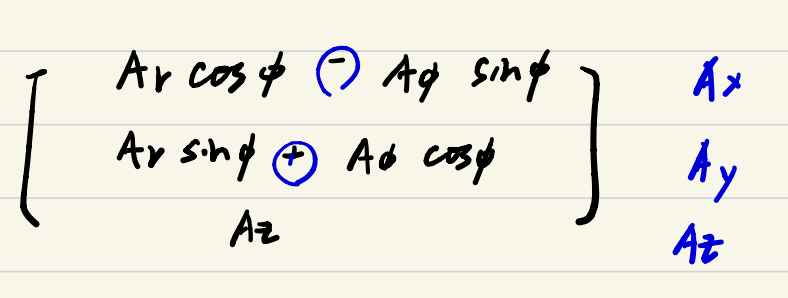
\includegraphics[width=0.7\linewidth]{1.png}
\end{figure}
\end{frame}
\begin{frame}{Spherical Coordinate}
\begin{itemize}
    \item Figure for Spherical Coordinate. Notice the position of $\phi, \theta$.
    \item
    $$
    (u_1, u_2, u_3) = (R, \theta, \phi)
    $$
    \item Right hand rule: 
    $$
    \vec{a_R} \times \vec{\theta} = \vec{\phi}
    $$
    \item $$
    \vec{A} = \vec{a_R}A_R + \vec{a_\theta}A_\theta + \vec{a_\phi}A_\phi
    $$
    \item differential length:
    \begin{equation}\label{Eq: spherical-differential-length}
        d\vec{l} = \vec{a_R}dR + \vec{a_\theta}Rd\theta + \vec{a_\phi}Rsin\theta d\phi
    \end{equation}, as $h_1 = 1, h_2 = R, h_3 = Rsin\theta$.
    \item differential area:
    $$
    ds_R = R^2sin\theta d\theta d\phi
    $$
\end{itemize}
\end{frame}
\begin{frame}{Spherical Coordinate}
\begin{itemize}
    \item differential volume: 
    $$
    dv = R^2 sin\theta dR d\theta d\phi
    $$
    \item conversion of quantities between Cartesian coordinate and Spherical coordinate:
    \begin{enumerate}
        \item
        $$
        \begin{cases}
            x = Rsin\theta cos\phi\\
            y = Rsin\theta sin\phi\\
            z = Rcos\theta
        \end{cases}
        $$
        \item
        $$
        \begin{cases}
            R=\sqrt{x^2+y^2+z^2}\\
            \theta = arctan\frac{\sqrt{x^2+y^2}}{z}\\
            \phi = arctan\frac{y}{x}
        \end{cases}
        $$
    \end{enumerate}
    \item From Spherical coordinate to Cartesian coordinate: represent $A_x$ by the quantities in Spherical coordinate; write the formula in the form of matrix. (Similar to cylindrical coordinate).
\end{itemize}
\end{frame}
\begin{frame}{Integral}
\begin{block}{Line integrals}
When integrated along a certain differential length, use equations we introduced last class to convert differential length to integrable quantities with regard to different coordinates. For example, in Cartesian coordinates, when integrating on $d\vec{l}$, you should convert $d\vec{l}$ into the form
$$d\vec{l} = \vec{a_x}dx + \vec{a_y}dy + \vec{a_z}dz.$$
\end{block}
\end{frame}
\begin{frame}{Integral}
\begin{block}{A small example}
Suppose $\vec{F}=\vec{a_x}xy - \vec{a_y}2x$, calculate its integral along $y=x^2$ in the range [0,1].
\end{block}
\pause 
\begin{block}{Answer}
\[
\begin{aligned}
W&=\int \vec{F}\cdot d\vec{l}\\
&=\int (\vec{a_x}xy - \vec{a_y}2x)\cdot (\vec{a_x}dx + \vec{a_y}dy)\\
&=\int xydx-2xdy\\
&=\int_0^1 (x*x^2dx-2x*2xdx)=-\frac{13}{12}\\
\end{aligned}
\]
\end{block}
\end{frame}
\begin{frame}{Integral}
Flux: the integrals of the vector field rush out the surface.
\begin{figure}[H]
	\centering
	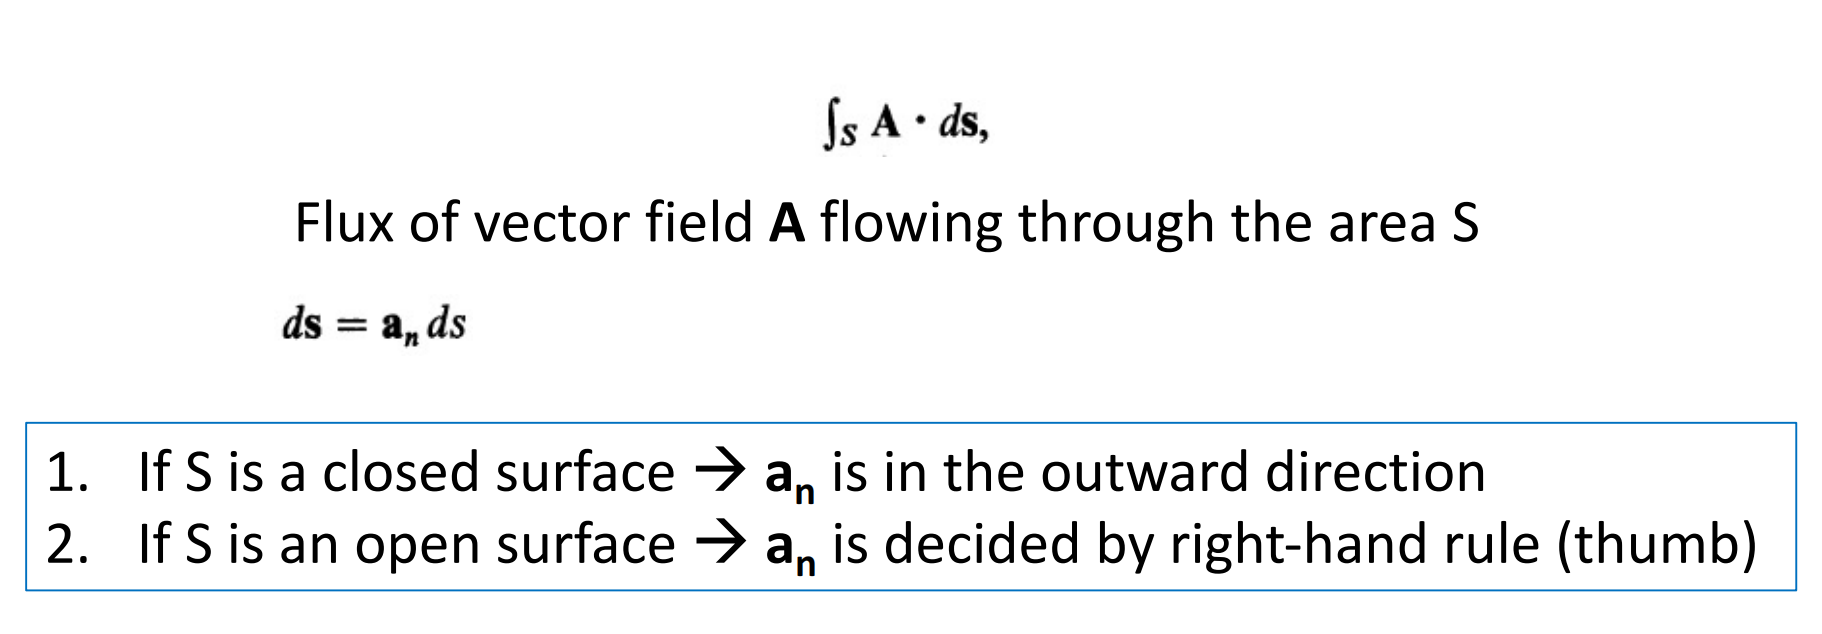
\includegraphics[width=0.7\linewidth]{2_1.png}
\end{figure}
\end{frame}
\begin{frame}{Scalar field and vector field}

\begin{block}{Scalar field}
The intensity of the field is a scalar value, for example, gravitation potential field.
\end{block}
\pause
\begin{block}{Vector field}
The intensity of the field is a vector value, for example, gravitational field.
\end{block}
\pause
\begin{block}{Connection}
The vector field can be the gradient of a scalar field. But it has some conditions: what conditions?
\end{block}
\end{frame}
\begin{frame}{Gradient of a scalar field}

\begin{itemize}
    \item $$\nabla V = \vec{a_n} \frac{dV}{dn}$$
    \item $\nabla V$ at certain point is a vector. Think about how can we represent $\nabla$ singly?
    \item $$dV = (\nabla V)\cdot d\vec{l}$$: the space rate of increase of $V$ in the $\vec{a_l}$ direction is equal to the projection (the component) of the gradient of $V$ in that direction. 
    \item $$
        \nabla V = \vec{a_{u1}} \frac{\partial V}{h_1\partial u_1} + \vec{a_{u2}}\frac{\partial V}{h_2\partial u_2} + \vec{a_{u3}} \frac{\partial V}{h_3\partial u_3}
    $$, when $V$ is taken off:
    $$
    \nabla \equiv  \vec{a_{u1}} \frac{\partial }{h_1\partial u_1} + \vec{a_{u2}}\frac{\partial }{h_2\partial u_2} + \vec{a_{u3}} \frac{\partial }{h_3\partial u_3}
    $$
\end{itemize}
\end{frame}
\begin{frame}{Divergence of a vector field}
\begin{itemize}
    \item divergence of a vector field $\vec{A}$ at a point $div\vec{A}$ as the net outward flux of $\vec{A}$ per unit volume as the volume about the point tends to zero: 
    \begin{equation}\label{Eq: definition-divergence-of-vector-field}
        div\vec{A} = \lim_{\Delta v\to 0}\frac{\oint\limits_{S}\vec{A}\,\mathrm{d}s}{\Delta v} 
    \end{equation}
 
    \item source: net positive divergence; sink: net negative divergence. zero divergence: no source/sink.
    \item $div\vec{A}$ at certain point is a scalar.
\end{itemize}

\end{frame}
\begin{frame}{Divergence of a vector field}
\begin{itemize}
    \item For Cartesian coordinate, 
    $$div\vec{A} = \frac{\partial A_x}{\partial x} + \frac{\partial A_y}{\partial y} + \frac{\partial A_z}{\partial z}$$
    \item $$\nabla \cdot \vec{A} \equiv div \vec{A}$$
    \item $$\nabla \cdot \vec{A} = \frac{1}{h_1h_2h_3}[\frac{\partial}{\partial u_1}(h_2h_3A_1)+\frac{\partial}{\partial u_2}(h_1h_3A_2)+\frac{\partial}{\partial u_3}(h_1h_2A_3)]$$
\end{itemize}
\end{frame}
\begin{frame}{Divergence Theorem}
\begin{itemize}
    \item $$\int_V\nabla\cdot \vec{A}dv = \oint_S\vec{A}\cdot d\vec{s}$$, the volume integral of the divergence of a vector field equals the total outward flux of the vector through the surface that bounds the volume.
    \item A most famous theorem in the physics - Gauss's law can be deduced by divergence theorem very easily. Thus, the divergence theorem will be quite fundamental in this course. Make sure you understand it.
\end{itemize}
\end{frame}
\begin{frame}{Curl of a vector field}
\begin{itemize}
    \item $$curl \vec{A}\equiv\nabla\times\vec{A}=\lim_{\Delta s\to 0}\frac{1}{\Delta s}[\vec{a_n}\oint_{C}\vec{A}\cdot d\vec{l}]_{max}$$: the curl of a vector field $\vec{A}$, denoted by $curl\vec{A}$ or $\nabla\times\vec{A}$, is a vector whose magnitude is the maximum net circulation of $\vec{A}$ per unit area as the area tends to zero and whose direction is the normal direction of the area when the area is oriented to make the net circulation maximum. (Right hand rule defines the positive normal to an area).
    \item $\nabla\times\vec{A}$ in a general coordinate:
    $$
    \nabla\times\vec{A}=\frac{1}{h_1h_2h_3}\begin{vmatrix}
        \vec{a_{u1}}h_1 & \vec{a_{u2}}h_2 &\vec{a_{u3}}h_3\\
        \frac{\partial}{\partial u_1} & \frac{\partial}{\partial u_2} &\frac{\partial}{\partial u_3}\\
        h_1A_1 & h_2A_2 & h_3A_3
    \end{vmatrix}
    $$
    \item curl-free vector field ($\nabla\times\vec{A}=0$): \textbf{irrotational} or \textbf{conservative field}, like the gravitation potential field.
\end{itemize}
\end{frame}
\begin{frame}{Stokes's Theorem}
\begin{itemize}
    \item $$\int_S(\nabla\times\vec{A})d\vec{s}=\oint_C\vec{A}\cdot d\vec{l}$$: the surface integral of the curl of a vector field over an open surface is equal to the closed line integral of the vector along the contour bounding the surface.
\end{itemize}
\end{frame}
\begin{frame}{Other Identities}
\begin{itemize}
    \item[I]
    \begin{itemize}
        \item $$\nabla\times(\nabla V) \equiv 0$$: the curl of the gradient of any scalar field is identically zero.
        \item Another interpretation: If a vector field is curl-free, it can be expressed as the gradient of a scalar field.
        \item Since a curl-free vector field is irrotational or conservative, an irrotational/conservative vector field can always be expressed as the gradient of a scalar field.
    \end{itemize} 
    \item[II]\begin{itemize}
        \item $$\nabla\cdot(\nabla\times\vec{A})\equiv0$$: the divergence of the curl of any vector field is identically zero.
        \item Another interpretation: if a vector field is divergenceless, it can be expressed as the curl of another vector field.
        \item Divergenceless field is called solenoidal field, which will be further discussed in later classes.
    \end{itemize}
\end{itemize}
\end{frame}
\begin{frame}{Other Identities}
\begin{block}{Laplacian in Cartesian Coordinates}
$$\nabla^2 V = \frac{\partial^2 }{\partial x^2}+\frac{\partial^2 }{\partial y^2}+\frac{\partial^2 }{\partial z^2}$$
\end{block}
\pause
\begin{block}{Helmholtz's Theorem}
Any vector in 3D can be decomposable into a sum of the following vector fields. A vector field (vector point function) is determined to within an additive constant if both its divergence and its curl are specified everywhere.
$$F=-\nabla V+\nabla\times A.$$
\end{block}
\end{frame}
\begin{frame}{Other useful vector properties}
\begin{figure}[H]
	\centering
	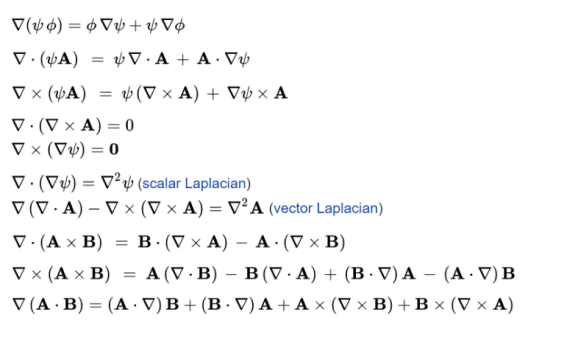
\includegraphics[width=0.9\linewidth]{2_3.png}
\end{figure}
\end{frame}



\end{document}